\documentclass[report.tex]{subfiles}

\begin{document}

\chapter{Antenna Part}

\section{\textit{LTE-M/NB-IoT} Antenna}

At the start of the project, the idea was to design a custom dipole antenna integrated into the watch strap. The design of a custom \textit{LTE-M/NB-IoT} antenna for the \textit{LTEWatch} was expected to be done but, due to the limited time available for the project and given the amount of work required to other tasks of the project, it was agreed with the project manager Medard Rieder to keep this part for further complementary tasks of this project. This is why this chapter only focuses on the design of the \textit{GNSS} antenna.

\section{\textit{GNSS} Antenna}

The \textit{LTEWatch} project integrates a \textit{GNSS} receiver which requires the implementation of a suitable \textit{GNSS} antenna. RF design applications and antenna integration are complex processes that require special attention. \textsc{u-blox} provides several documentations about RF design and antenna integration process. The following sections are based on the following list of documentation and application note from \textsc{u-blox}:
\begin{enumerate}
\item \textit{"RF design considerations for u-blox GNSS receivers"} (src.\cite{gnss_ant_intro})
\item \textit{"Antenna integration guidance"} (src.\cite{gnss_antenna_integr})
\item \textit{"Design guide for small, high performance GNSS patch antenna applications"} (src.\cite{gnss_patch_antenna})
\end{enumerate}
\subsection{Introduction to \textit{GNSS} Antenna Integration}

\textit{GNSS} applications have become very common in wearable and compact embedded applications. Applications that need to be more and more compact while increasing battery life and performance, in addition to an environment crowded with RF signals of all kinds. Due to these constraints, antennas are a critical part of any \textit{GNSS} receiver design that requires special attention. As explained earlier, \textit{GNSS} signals are extremely weak and even an optimal receiver cannot compensate for a bad antenna or in-band interference due to poor RF board design. Therefore, antenna integration plays an important role in the performance of \textit{GNSS} applications.

\subsection{Antenna basics}
\subsubsection{General considerations:}

In \textit{GNSS} applications, a good sky visibility is crucial, more satellites \textit{GNSS} signal reception by the \textit{GNSS} receiver means more performance and accuracy. Conversely, poor sky visibility environments such as narrow streets, underground parking lots, or any object covering the antenna will cause position drift and a significantly longer \textit{TTFT} (\textit{Time To First Fix}), resulting in more power consumption and less battery life. A \textit{GNSS} receiver can only achieve its specified performance if the \textit{average carrier to noise power density ratio} of the strongest satellites reach at least \SI{44}{\decibel\hertz}. In an optimal RF design, the average of the $C/N_0$ ratio of high elevation satellites should be in the following range:
$$
	\boxed{ \SI{44}{\decibel\hertz} \leq \dfrac{C}{N_0} \leq \SI{50}{\decibel\hertz}} \quad  \dfrac{C}{N_0}\textit{ : Average carrier to noise power density ratio}
$$

\subsubsection{\textit{GNSS} Antenna Requirements:}
To achieve optimal performance, the \textit{GNSS} antenna should fulfill the following requirements:
\begin{enumerate}
\item Use high gain antenna: $>\SI{4}{\decibel ic}$
\item With active antenna, use \textit{LNA} with low noise figure: $< \SI{2}{\decibel}$
\item Low level of directivity: As shown in figure \ref{fig:low_direct_gnss}
\item Good sky visibility
\item Good matching between antenna and RF line impedance
\item High gain
\item Filter
\end{enumerate}

\begin{figure}[H]
	\centering
	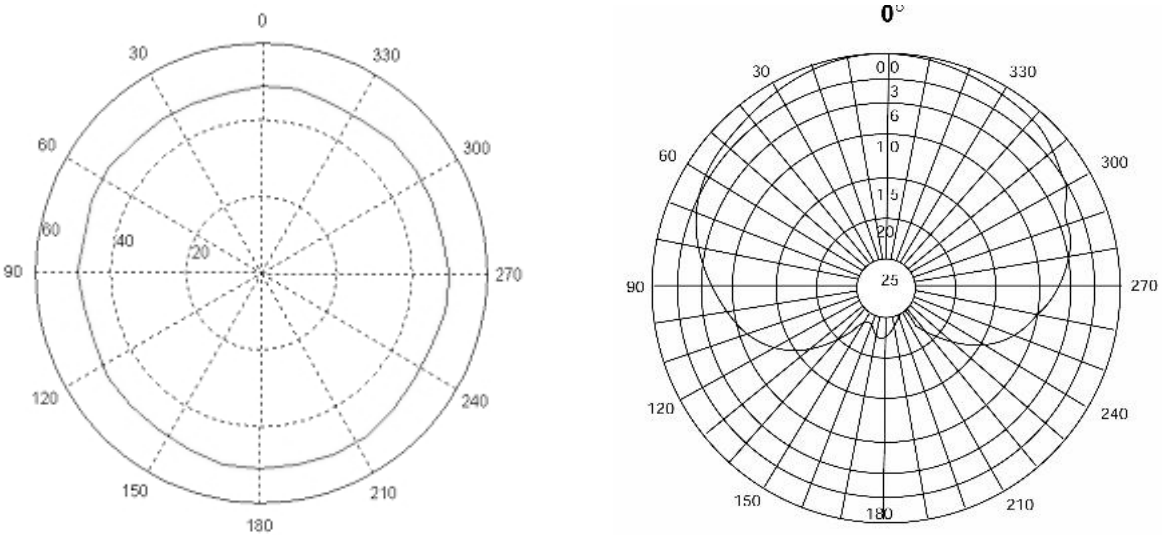
\includegraphics[width=0.8\textwidth]{Include/Figure/antenna/low_direct_gnss.png}
	\caption{Low directivity (left), high directivity (right) - Source:\cite{gnss_ant_intro}}
	\label{fig:low_direct_gnss}
\end{figure}

\subsection{Active vs. Passive Antenna}

Antennas are available in two main categories :
\begin{enumerate}
\item Passive antennas (ceramic patch, helix structure): 
\begin{itemize}
\item Only contain the radiating element
\item Can also contain a \SI{50}{\ohm} line impedance adaptation matching network
\end{itemize}
\pagebreak
\item Active antennas
\begin{itemize}
\item Integrated \textit{LNA} (\textit{Low Noise Amplifier})
\begin{itemize}
\item Eliminate the line losses after the \textit{LNA} which reduce the overall noise
\item Reduce the overall noise figure of the system resulting in better sensitivity
\end{itemize} 
\item Some receivers require active antenna only
\item Increase power consumption $\boxed{3 \ldots \SI{20}{\milli\ampere}}$\\
\end{itemize}
\end{enumerate}

Active antennas are always advisable if antenna receiver line length exceeds $\boxed{\SI{10}{\centi\meter}}$. The gain of the \textit{LNA} inside the antenna must not lead to an overload condition at the receiver. For receivers that also work with passive antennas an antenna LNA gain of $\boxed{\SI{15}{\decibel}}$ is usually sufficient, even for cable lengths up to $\SI{5}{\meter}$. There is no need for the antenna \textit{LNA} gain to exceed $\boxed{\SI{26}{\decibel}}$ for use with \textsc{u-blox} receivers (at the RF input). With shorter cables and a gain above $\boxed{\SI{35}{\decibel}}$, an overload condition might occur on some receivers.\\

When comparing the gain figures of active and passive antennas, keep in mind that the gain of an
active antenna is composed of two components :
\begin{enumerate}
\item \textbf{Antenna gain of the passive radiator} : given in \si{\decibel ic}
\item \textbf{\textit{LNA} power gain} : given in \si{\decibel}\\
\end{enumerate}

A low antenna gain cannot be compensated by high \textit{LNA} gain. \textbf{It is not possible to judge the quality of the antenna if a manufacturer provides only one total gain figure}. Information on the antenna gain (in \si{\decibel ic}), the amplifier gain, and the amplifier noise figure is also required.

\begin{table}[H]
\centering
\begin{tabularx}{\textwidth}{|X|X|}\hline
\textbf{Active antenna} & \textbf{Passive antenna}\\\hline\hline
Needs more power ($10 - \SI{60}{\milli\watt}$) than a passive antenna   & Does not add anything to the power budget \\\hline
Is more tolerant to minor impedance miss-match or cable length than a passive antenna & Antenna must be connected with a carefully designed micro strip or strip line of maximum \SI{10}{\centi\meter} to the \textit{GNSS} receiver to ensure good \textit{GNSS} performance \\\hline
Helps to keep the receiver noise figure low & Jamming signals coupled into the micro-strip or strip line negatively affect the performance \\\hline
Is less affected by jamming into the antenna cable than a passive antenna (if equipped with filter) & RF design experience is required to properly design a passive antenna \\\hline
\end{tabularx}
\caption{Active vs Passive antenna table - Source:\cite{gnss_ant_intro}}
\label{tab:modem}
\end{table}

\subsection{Passive \textit{GNSS} Antennas:}

It is important to know that \textit{GNSS} signal is right-hand circuit polarized (RHCP) which result in different needs of antenna style than the well-known \textit{whip} antenna used for linear polarized signals.\\

For \textit{GNSS} application, the list of available antenna style is the following:
\begin{itemize}
\item Patch Antenna
\item Helix Antenna
\item Monopole Antenna
\begin{itemize}
\item Chip Antenna
\item PCB Antenna
\item Fractal Element Antenna (FEA)
\end{itemize}
\item Dipole antenna
\begin{itemize}
\item Loop antenna
\item Planar Inverted F Antenna (PIFA)
\item High-end GNSS antennas
\end{itemize}
\end{itemize}

\subsubsection{Patch Antenna:}
\begin{itemize}
\item Most common antenna for \textit{GNSS} applications
\item Flat antenna
\item Have a ceramic and metal body mounted on a metal base plate
\item Often cast in housing
\end{itemize}

\begin{figure}[H]
	\centering
	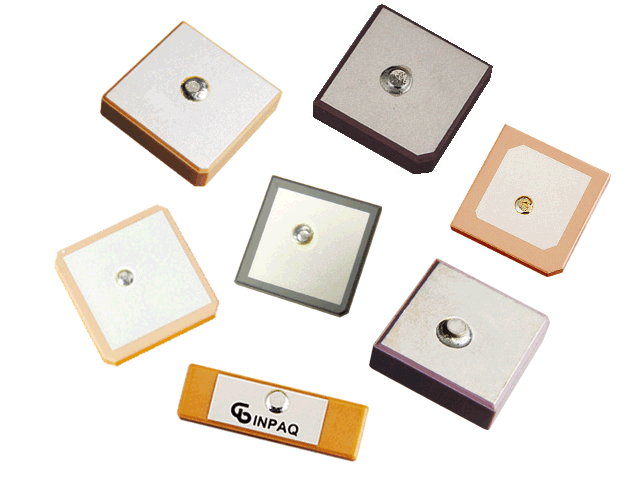
\includegraphics[width=0.35\textwidth]{Include/Figure/antenna/patch_antenna_1.png}
	\caption{Example of patch antenna - Source:\url{https://www.inpaq.com.tw/upload/file/20160125020258534235875.png}}
	\label{fig:patch_antenna_1}
\end{figure}

\begin{flushleft}
\textbf{Advantages:}
\end{flushleft}
\begin{itemize}
\item Ideal for flat surface mounting
\item Very high gain capable
\item Low cost
\item Huge variation of available size ($40\times \SI{40}{\milli\meter}$ down to $10\times \SI{10}{\milli\meter}$)
\end{itemize}

\begin{flushleft}
\textbf{Disadvantages:}
\end{flushleft}
\begin{itemize}
\item Require a large ground plane for best performance ($70\times \SI{70}{\milli\meter}$)
\item A smaller antenna equal a lower overall gain
\item Amplifying the signal after the antenna will not improve the \textit{SNR} (\textit{Signal to Noise Ratio})
\item The minimal ground plane size is ($50\times \SI{50}{\milli\meter}$)
\end{itemize}

\begin{flushleft}
\textbf{Practical values:}
\end{flushleft}
\begin{enumerate}
\item Patch antennas size $= 25 \times \SI{25}{\milli\meter}$ :
\begin{itemize}
\item Optimal performance
\item Cost-efficient
\end{itemize}
\item Patch antennas size $< 17 \times \SI{17}{\milli\meter}$ :
\begin{itemize}
\item Moderate navigation performance (Unless enhanced by \textsc{u-blox} \textit{SuperSense technology})
\end{itemize}
\end{enumerate}

\warning{\textbf{Performance is highly dependent to the ground plane size}}

\subsubsection{Helix Antenna:}

\begin{itemize}
\item Geometric size depends on the dielectric that fill the space between the active parts of the antenna
\item Air dielectric : Large dimension ($l = \SI{60}{\milli\meter}$, $\oslash = \SI{45}{\milli\meter}$)
\item Ceramic dielectric: Much smaller form factor
\end{itemize}

\begin{figure}[H]
	\centering
	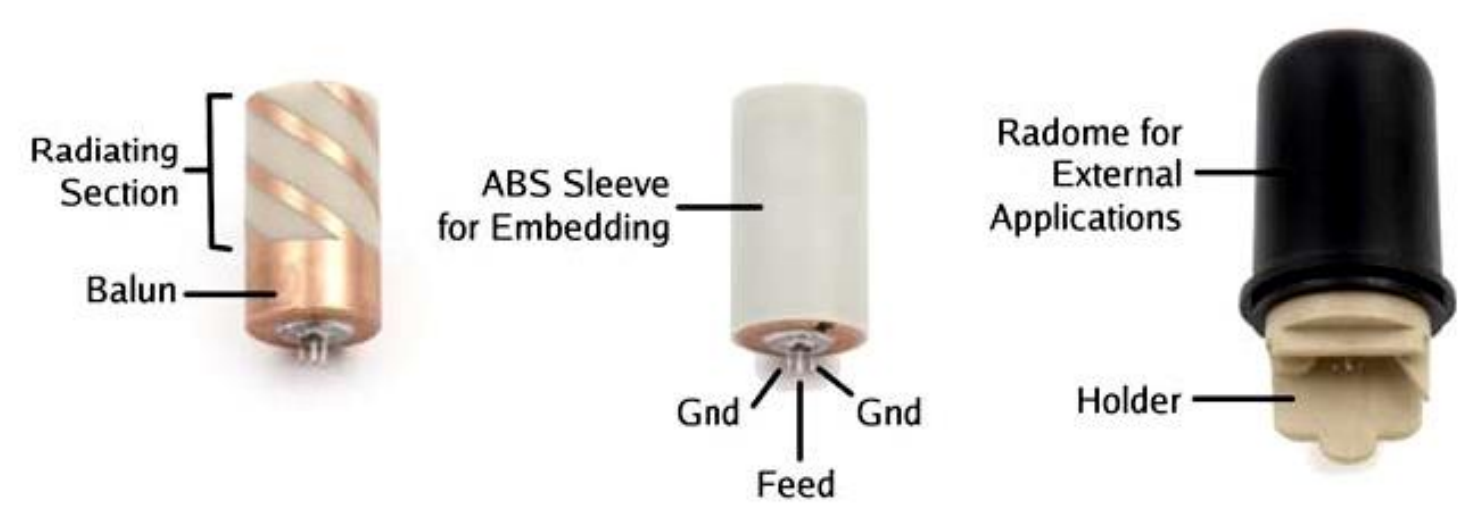
\includegraphics[width=0.5\textwidth]{Include/Figure/antenna/helix_ant.png}
	\caption{Example of helix antenna - Source:\cite{gnss_ant_intro}}
	\label{fig:helix_ant}
\end{figure}

\begin{flushleft}
\textbf{Advantages:}
\end{flushleft}
\begin{itemize}
\item Like patch antennas, filling the antenna with a high dielectric constant material can reduce the size of helix antennas
\item Antenna size of $l=\SI{18}{\milli\meter}$ and $\oslash = \SI{10}{\milli\meter}$ are being available on the market
\end{itemize}

\begin{flushleft}
\textbf{Disadvantages:}
\end{flushleft}
\begin{itemize}
\item Smaller antenna dimensions $\rightarrow$ tight manufacturing tolerances
\item Antenna gain decrease with size of the antenna
\end{itemize}

\subsubsection{Monopole Antenna - Chip Antenna:}
\begin{itemize}
\item More and more common for compact \textit{GNSS} designs
\item Very common smart-phone and \textit{Personal-Navigation-Devices }(\textit{PNDs}) applications
\end{itemize}

\begin{figure}[H]
	\centering
	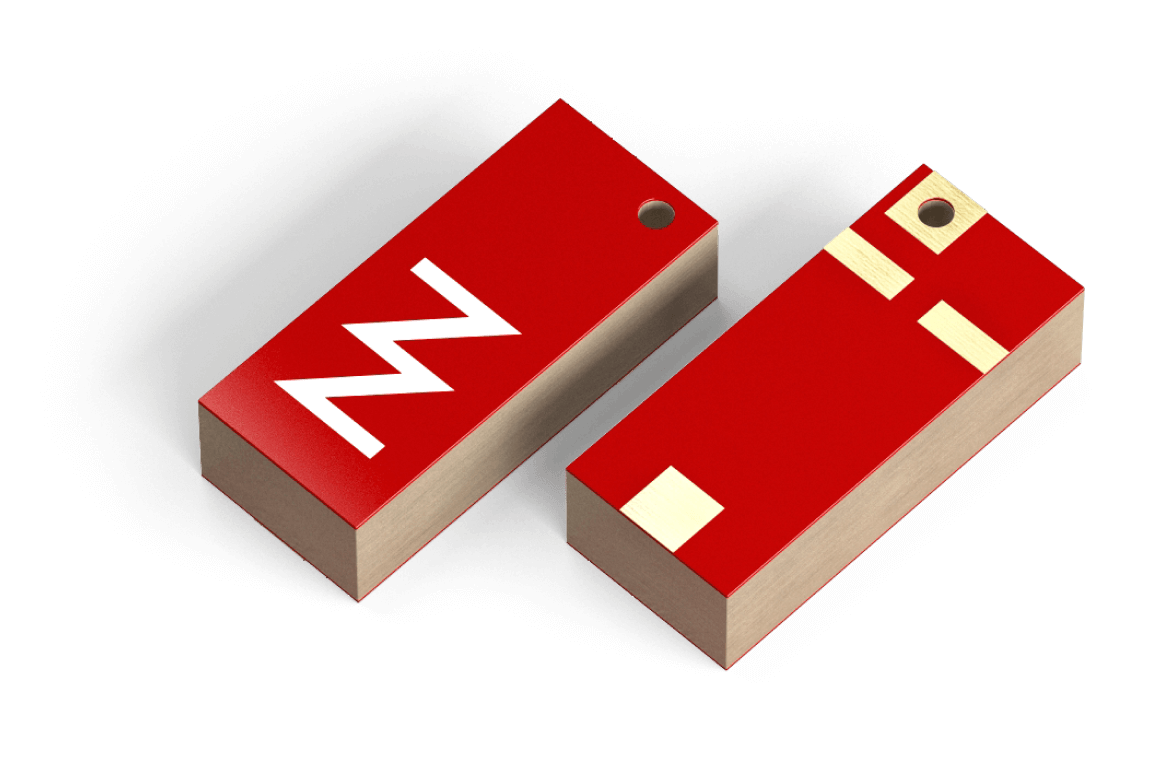
\includegraphics[width=0.4\textwidth]{Include/Figure/antenna/chip_antenna.png}
	\caption{Example of chip antenna - Source: \url{https://ignion.io}}
	\label{fig:chip_antenna}
\end{figure}

\begin{flushleft}
\textbf{Advantages:}
\end{flushleft}
\begin{itemize}
\item Low cost
\item Extremely small size available ($3.2\times 1.6 \times \SI{1.1}{\milli\meter}$)
\item High gain
\item Omni-directional radiation patterns
\end{itemize}

\begin{flushleft}
\textbf{Disadvantages:}
\end{flushleft}
\begin{itemize}
\item A variety of factors influence their performance due to their miniature size
\begin{itemize}
\item Footprint
\item Ground plane size
\item Isolation distance (typ. $\SI{5}{\milli\meter}$) : The keep-out area can have an important impact on antenna efficiency and \textit{GNSS} performance
\end{itemize}
\item Require more careful RF design
\item Respecting all recommendations doesn't guaranty performance due to potential detuning effects created by nearby objects
\end{itemize}

\begin{flushleft}
\textbf{Practical recommendations:}
\end{flushleft}
\begin{itemize}
\item Even if the antenna manufacturers claim that a ground plane is not required, the available ground plane has a significant impact on the \textit{GNSS} performance of a chip antenna. Therefore, not only the size of the chip but also the ground plane must be considered in the design. For designs with a sufficiently large ground plane a chip antenna can provide satisfactory \textit{GNSS} performance. 
\item  However, in designs with an inadequate ground plane and device layout their performance is insufficient for \textit{GNSS}.
\item  Chip antennas have a $\SI{3}{\decibel}$ loss compared to helical or patch antennas due to linear polarization and their performance is highly dependent on the size of the ground plane
\item  Chip antennas are not recommended for use in devices where navigation is an essential feature
\end{itemize}

\subsubsection{Monopole Antenna - PCB Antenna:}

\begin{flushleft}
\textbf{Advantages:}
\end{flushleft}
\begin{itemize}
\item Simple and economical antenna solution
\item Cheapest \textit{GNSS} antenna solution
\item Usually have a larger bandwidth than chip or patch antennas
\end{itemize}

\begin{figure}[H]
	\centering
	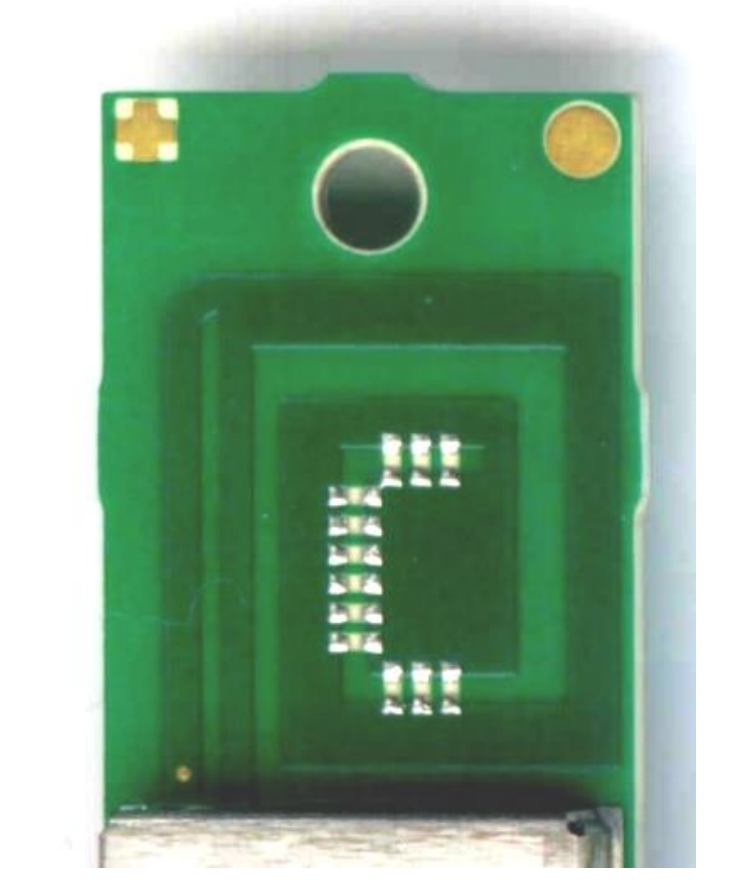
\includegraphics[width=0.3\textwidth, angle=90]{Include/Figure/antenna/pcb_antenna.png}
	\caption{Example of \textit{PCB} antenna - Source:\cite{gnss_ant_intro}}
	\label{fig:pcb_antenna}
\end{figure}

\begin{flushleft}
\textbf{Disadvantages:}
\end{flushleft}
\begin{itemize}
\item Significantly weaker signals compared to a patch or helix antennas
\item Loss of $-3\si{\decibel}$ due to linear polarization
\item Massively in-homogeneous directivity
\item Lower overall gain
\item Typically bigger than chip antennas
\item Requires RF expertise
\end{itemize}

\subsubsection{Dipole Antenna:}

\begin{flushleft}
\textbf{Advantages:}
\end{flushleft}
\begin{itemize}
\item Very cost-effective solution, especially when printed on PCB
\item Acceptable performance in indoor environments
\item Field independent from any ground plane
\item Linear polarization increase \textit{backlog} sensitivity which is useful for indoor reception
\end{itemize}

\begin{figure}[H]
	\centering
	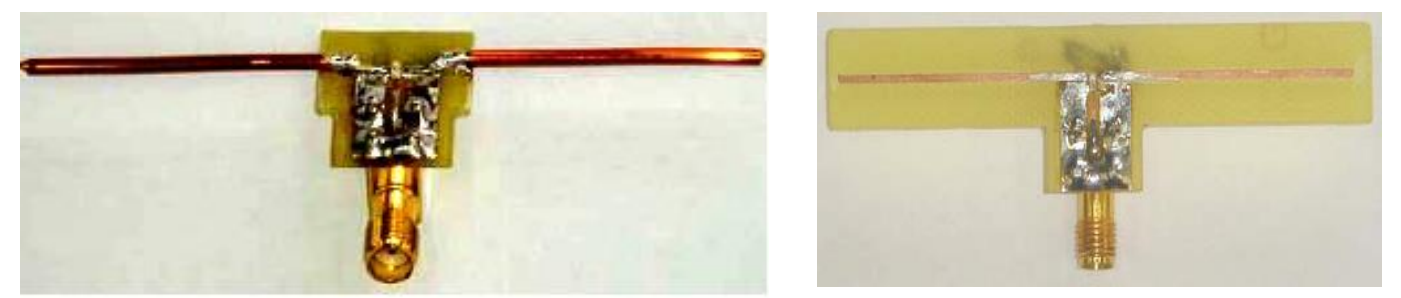
\includegraphics[width=0.9\textwidth]{Include/Figure/antenna/dipole_antenna.png}
	\caption{Example of dipole antennas - Source:\cite{gnss_ant_intro}}
	\label{fig:dipole_antenna}
\end{figure}
  
\begin{flushleft}
\textbf{Disadvantages:}
\end{flushleft}
\begin{itemize}
\item Linear polarized antenna: $\SI{3}{\decibel}$ loss for \textit{GNSS} in open spaces
\item Similar drawbacks as PCB antennas
\item Require RF expertise
\end{itemize}

\begin{flushleft}
\textbf{Practical recommendations:}
\end{flushleft}
\warning{\textbf{Warning: }Dipole antennas are not recommended for use in devices where navigation is an essential feature}

\subsubsection{Dipole Antenna - Loop antenna:}

\begin{figure}[H]
	\centering
	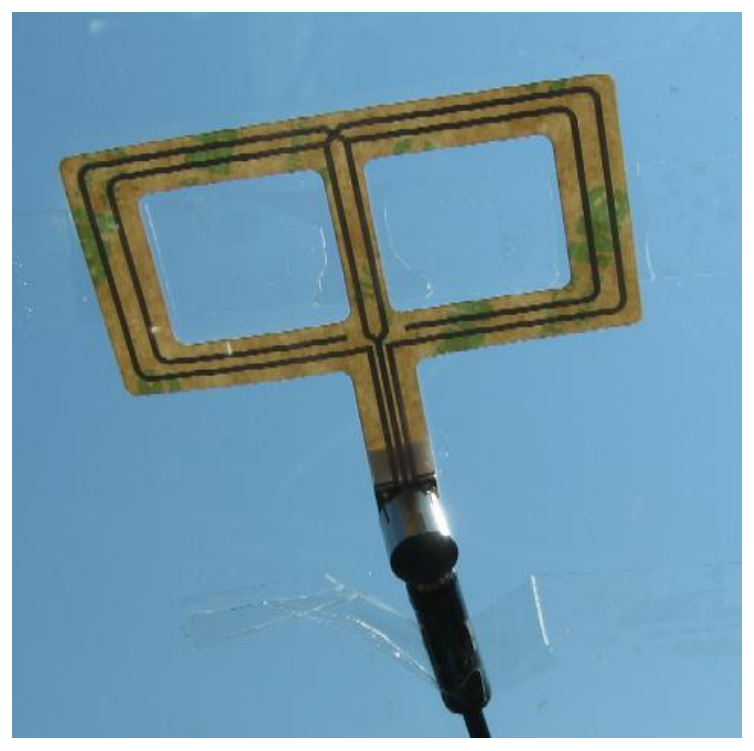
\includegraphics[width=0.4\textwidth]{Include/Figure/antenna/loop_antenna.png}
	\caption{Example of dipole loop antenna - Source:\cite{gnss_ant_intro}}
	\label{fig:loop_antenna}
\end{figure}

\begin{flushleft}
\textbf{Advantages:}
\end{flushleft}
\begin{itemize}
\item Independent from ground plane $\rightarrow$ not sensitive to objects in the near field
\item  Good navigation performance when mounted on glass 
\end{itemize}

\begin{flushleft}
\textbf{Disadvantages:}
\end{flushleft}
\begin{itemize}
\item Not a suitable solution for small embedded system
\end{itemize}

\subsubsection{Dipole Antenna - Planar Inverted F Antenna (PIFA):}

\begin{figure}[H]
	\centering
	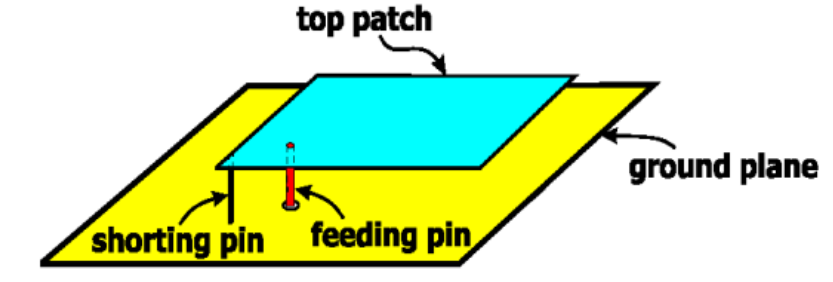
\includegraphics[width=0.5\textwidth]{Include/Figure/antenna/pifa_antenna.png}
	\caption{Example of dipole \textit{PIFA} antenna - Source:\cite{gnss_ant_intro}}
	\label{fig:pifa_antenna}
\end{figure}

\pagebreak

\begin{flushleft}
\textbf{Advantages:}
\end{flushleft}
\begin{itemize}
\item Suitable antenna solution for embedded applications
\item Nearly omnidirectional 
\item Multi-band radiation capability
\end{itemize}

\begin{flushleft}
\textbf{Disadvantages:}
\end{flushleft}
\begin{itemize}
\item Linearly polarized : $\SI{3}{\decibel}$ loss
\item Only moderate efficiency
\end{itemize}

\begin{flushleft}
\textbf{Practical recommendations:}
\end{flushleft}
\begin{itemize}
\item Mainly used in cellular phones (\textit{E-911}) applications
\item Not recommended for applications where navigation is an essential feature
\end{itemize}

\subsubsection{Dipole Antenna - High-end \textit{GNSS} antennas:}

\begin{flushleft}
\textbf{Advantages:}
\end{flushleft}
\begin{itemize}
\item Highly optimized for multi-path reflected signals suppression (choke ring antennas, multi-path limiting antennas, \textit{MLA})
\item Very accurate antenna phase center determination
\end{itemize}

\begin{flushleft}
\textbf{Disadvantages:}
\end{flushleft}
\begin{itemize}
\item Larger size
\item Higher power consumption
\item Higher price
\end{itemize}

\begin{flushleft}
\textbf{Practical recommendations:}
\end{flushleft}
\begin{itemize}
\item Recommended for precision \textit{GNSS} applications with position resolution in the \si{\milli\meter} range
\item For that kind of application, it is required that signals from all elevations  satellites meet at exactly the same point inside the antenna
\item Receivers with multiple antenna inputs are often required for that kind of precision
\end{itemize}

\pagebreak

\subsection{\textit{LTEWatch} \textit{GNSS} Antenna Selection}

Considering all points described in previous sections, the best solution for the \textit{LTEWatch} \textit{GNSS} receiver seems to be a passive chip antenna. After long research on available solution on the market, a suitable solution was found: the \textit{DUO mXTEND (NN03-320)} from \textsc{ignion}.

\subsubsection{\textit{DUO mXTEND (NN03-320)} from \textsc{ignion}:}

\begin{figure}[H]
	\centering
	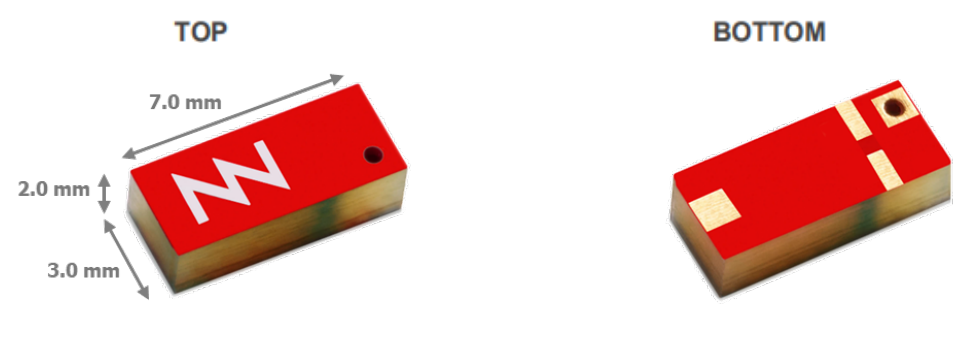
\includegraphics[width=0.7\textwidth]{Include/Figure/antenna/gnss_antenna.png}
	\caption{\textit{DUO mXTEND (NN03-320)} Antenna from \textsc{ignion} - Source:\cite{GNSSANT}}
	\label{fig:gnss_antenna}
\end{figure}

The datasheet of the \textit{DUO mXTEND (NN03-320)}\cite{GNSSANT} describes the antenna as a versatile product can be used to operate communication services such as, \textit{5G}, \textit{GNSS}, \textit{BT}, \textit{Wi-Fi}, or \textit{UWB} in a \textit{single port }or \textit{multiport} configuration.\\

\begin{flushleft}
The \textit{NN03-320} is designed for application such as:
\end{flushleft}
\begin{itemize}
\item \textit{UWB} modules
\item Smart Watches
\item Air Tags
\item Earphones
\item Bluetooth modules
\item Asset Trackers
\end{itemize}

\begin{flushleft}
\textbf{Features \& Benefits:}
\end{flushleft}
\begin{itemize}
\item Multipurpose: Multiband \textit{IoT} chip antenna component with multiport (2 independant ports)
\item Low power consumption
\item High efficiency
\item Smallest clearance: No clearance beyond the antenna footprint
\item Miniature: Ultra compact form factor of $\SI{7.0}{\milli\meter} \times \SI{3.0}{\milli\meter} \times \SI{2.0}{\milli\meter}$
\item Best for combining : One or more GNSS, Bluetooth, UWB and 5G applications.
\item Versatile: Can be mounted on device center edge or on device corner
\item Reliability: \textit{Off-the-Shelf} standard product
\end{itemize}

\subsubsection{Antenna Design Tool from \textsc{ignion} \textit{(Antenna Intelligence Cloud)}:}

One of the biggest advantages of anntenna solution from \textsc{ignion} is that they provides an online antenna design tool \textit{"Antenna Intelligence Cloud"} on their website: \url{https://ignion.io/antenna-intelligence/}. This tools allow to get a RF design proof of concept in \SI{24}{\hour} and also provides a full simulation of a custom design with performance values, electrical schematic and components selection.

\subsubsection{\textit{LTEWatch} \textit{GNSS} Antenna:}

For the \textit{LTEWatch}, I asked for a custom wearable application design using \textit{LTE-M/NB-IoT} and \textit{GNSS} communication standard on a $\SI{40}{\milli\meter} \times \SI{40}{\milli\meter}$ board. A document containing a design proposition was received. The full document is available in appendix \ref{appendix:LTEWatch_NNS1} and the main specifications of the proposed solution by \textsc{Ignion} are illustrated in figures \ref{fig:ignion}
to \ref{fig:ignion_gnss_perf}.\\

\textbf{Figure \ref{fig:ignion} illustrates the \textit{GNSS} Antenna placement proposition:}

\begin{figure}[H]
\centering
\begin{subfigure}{.65\textwidth}
	\centering
	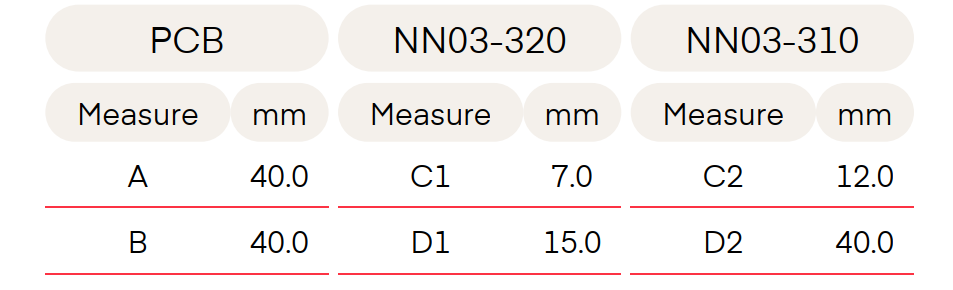
\includegraphics[width=1\textwidth]{Include/Figure/antenna/ignion_2.png}
\end{subfigure}
\begin{subfigure}{.55\textwidth}
	\centering
	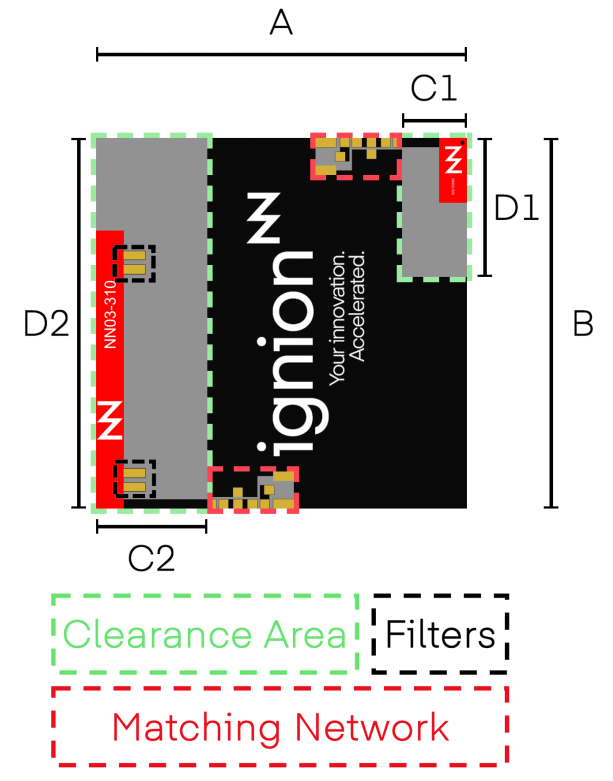
\includegraphics[width=1\textwidth]{Include/Figure/antenna/ignion_1.png}
\end{subfigure}
	\caption{Sketch of the proposed antenna placement and clearance}
	\label{fig:ignion}
\end{figure}

\textbf{Figure \ref{fig:gnss_antenna} illustrates the \textit{GNSS} antenna matching network topology:}

\begin{figure}[H]
	\centering
	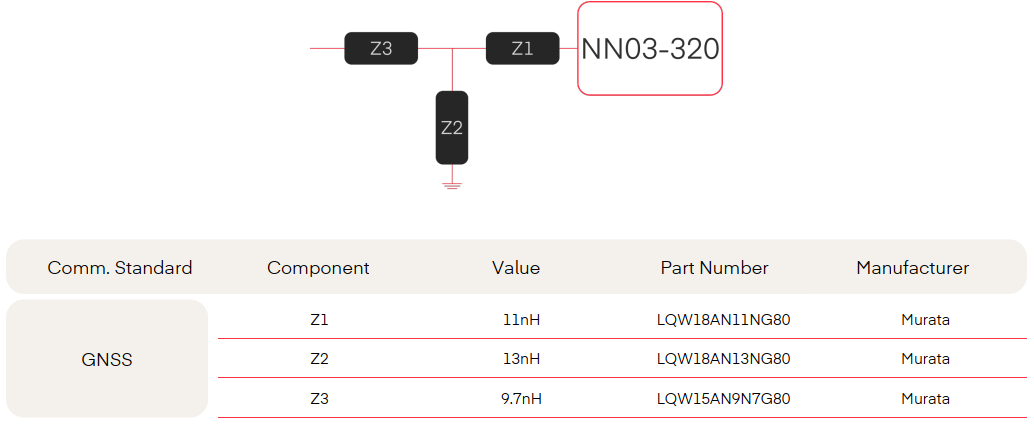
\includegraphics[width=0.9\textwidth]{Include/Figure/antenna/ignion_gnss.png}
	\caption{\textit{GNSS} Matching Network topology proposed by \textsc{Ignion}}
	\label{fig:gnss_antenna}
\end{figure}

\textbf{Figure \ref{fig:ignion_gnss_perf} illustrates the expected performance proposed by \textsc{Ignion}:}

\begin{figure}[H]
\centering
\begin{subfigure}{1\textwidth}
	\centering
	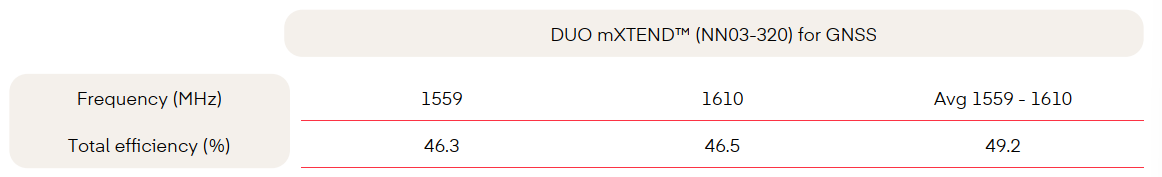
\includegraphics[width=1\textwidth]{Include/Figure/antenna/ignion_gnss_perf_2.png}
\end{subfigure}
\begin{subfigure}{0.75\textwidth}
	\centering
	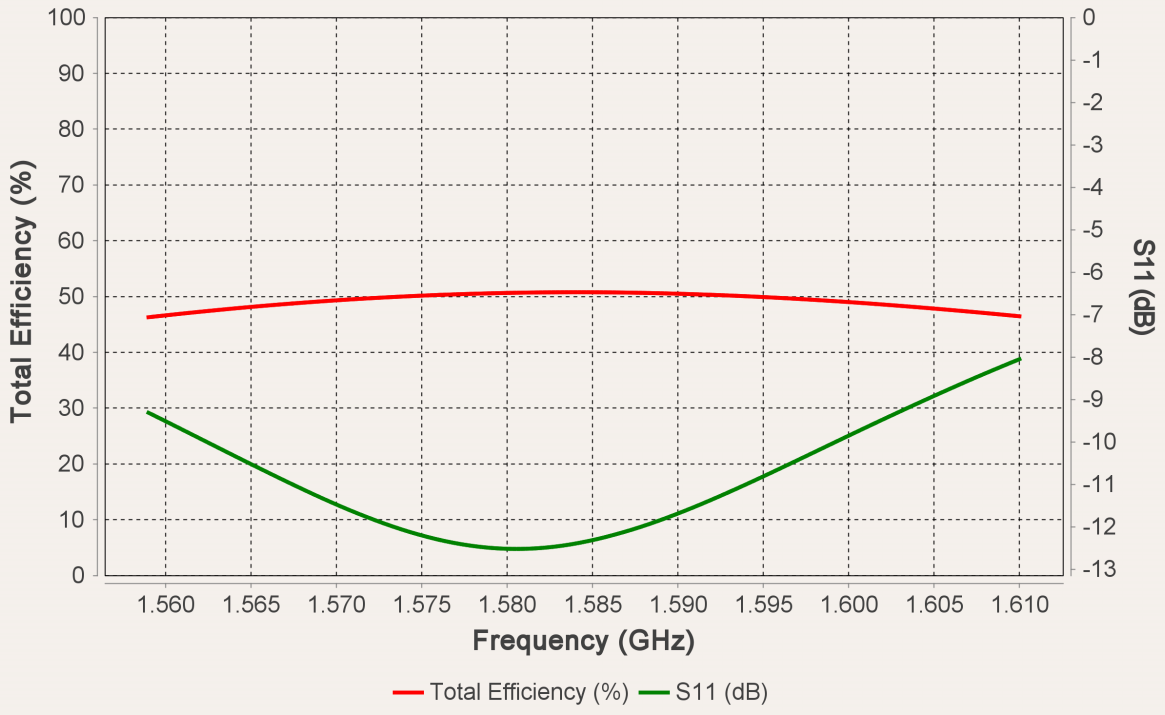
\includegraphics[width=1\textwidth]{Include/Figure/antenna/ignion_gnss_perf.png}
\end{subfigure}
	\caption{Expected device performance for the proposed design by \textsc{Ignion}}
	\label{fig:ignion_gnss_perf}
\end{figure}

As shown in figure \ref{fig:ignion_gnss_perf}, the expected performance of the proposed solution is not very impressive but is not that bad considering the very limited size of the ground plane. An efficiency of \SI{50}{\percent} is not optimal but still sufficient for a small \textit{GNSS} application. It is also important to mention that the \textit{LTEWatch} prototype board has a much larger size and a much larger ground plane. \textsc{Ignion} specifies in the documentation that an increase \SI{10}{\milli\meter} in board length results in an improvement in total efficiency of \SI{0.5}{\decibel}, of this fact, we can expect a significantly higher total efficiency with the \textit{LTEWatch} prototype board.









\end{document}
